\chapter{Evaluation}
\ifpdf
    \graphicspath{{Evaluation/EvaluationFigs/PNG/}{Evaluation/EvaluationFigs/PDF/}{Evaluation/EvaluationFigs/}}
\else
    \graphicspath{{Evaluation/EvaluationFigs/EPS/}{Evaluation/EvaluationFigs/}}
\fi

\section{Comparison of Analysis Results to Theory}
A major goal of this project is to show that the structure and content of types of poetry can be derived by analysing corpuses of collections. We would like to investigate how our results matches up with those documented in literary theory, as described by Young Writers\cite{youngwriters}, a poetry and creative writing resource for UK schools, and poets.org\cite{poetsorg}, supported by the Academy of American Poets.

We evaluate the results of analysing 450 limericks, 718 haiku and all 154 of Shakespeare's sonnets. These three types of poetry cover a large range of techniques and are of varying lengths, enabling us to evaluate more completely.

\subsection{Limericks}

\begin{description}
\item[One stanza, five lines, no repetition]  \hfill \\
All of the poems in our corpus follow this rule, as seen in Figure \ref{fig:lim1}.
\begin{figure}[H]
\centering
\begin{subfigure}[t]{0.3\textwidth}
	\centering
    \includegraphics[width=50mm]{lim-stanza}
    \caption{Just one stanza}
    \label{fig:lim-stanza}
\end{subfigure}
\begin{subfigure}[t]{0.3\textwidth}
	\centering
    \includegraphics[width=50mm]{lim-lines}
    \caption{Always five lines}
    \label{fig:lim-lines}
\end{subfigure}
\begin{subfigure}[t]{0.3\textwidth}
	\centering
    \includegraphics[width=50mm]{lim-rep-lines}
    \caption{No lines are repeated}
    \label{fig:lim-rep-lines}
\end{subfigure}
\caption{One stanza, five lines, no repetition.}
\label{fig:lim1}
\end{figure}


\item[Usually begins with \textit{'There was a...'} and ends with a name, person or place]  \hfill \\
Figure \ref{fig:lim-grams1} shows the N-Grams for line 1. We can see that \textit{'There be a young'}, the lemmatised version of \textit{'There was a'} with the added \textit{'young'} adjective is used with significant frequency (any substring is also considered a significantly frequent n-gram). We can also see in Figure \ref{fig:lim-anim} that limericks largely talk about animate objects (such as people) or non-objects (such as places). Furthermore, Figure \ref{fig:lim-types} confirms that the type of persona are people, organisms and animals.

\begin{figure}[H]
\centering
\includegraphics[width=140mm]{lim-grams1}
\caption{N-grams for Line 1}
\label{fig:lim-grams1}
\end{figure}

\begin{figure}[H]
\centering
\includegraphics[width=120mm]{lim-anim}
\caption{Animation of nouns}
\label{fig:lim-anim}
\end{figure}

\begin{figure}[H]
\centering
\includegraphics[width=120mm]{lim-types}
\caption{Types of persona}
\label{fig:lim-types}
\end{figure}

Overall, our results supports the theory. However, since the analysis omits Named Entity Recognition, we are unable to specifically say whether or not it was a person or a place.

Furthermore, our results only show that 52 poems have this n-gram, which is only 11.6\% of the corpus. We suspect this discrepancy comes from the popularity of Edward Lear poems, of which most start with \textit{'There was a...'}, but poems by other authors do not generally use this as a rule. This comes down to the contents of the corpus. Since it was a collection of previously unseen poems from various sources across the Internet, we do not know the proportion of Edward Lear poems in the corpus before analysis (as required to avoid biasing the corpus as mentioned in Section \ref{sec:corpus}). If the poem had a higher proportion of Edward Lear limericks, the frequency of this property would probably increase. However, since we are analysing limericks in general, our result may be representative.

\item[Last line is farfetched or unusual]  \hfill \\
We have no way of determining this from our analysis or results because the social context of the poem was never considered. As a result this feature will only occur by chance during generation, not intention.

\item[Usually nonsense or humour]  \hfill \\
As above.

\item[\textit{AABBA} rhyme scheme]  \hfill \\
Our results show that this is by far the most probable rhyme scheme, as seen in Figure \ref{fig:lim-rhyme}. The other possibilities are close variations of \textit{AABBA}, eluding to the limitations of the CMU Pronunciation Dictionary and our method of handling words unknown to it, as described in Section \ref{sec:phonetic}. The results may yet improve if we were to build a state transducer model to predict the most likely rhythm pattern for words that are not in the dictionary.

\begin{figure}[H]
\centering
\includegraphics[width=140mm]{lim-rhyme}
\caption{Rhyme Scheme}
\label{fig:lim-rhyme}
\end{figure}

Despite those shortcomings the results follow Zipf's law as discussed in Section \ref{sec:overall-struct}, which means that we can treat the top result as unambiguous. Therefore, all limericks generated by the system will aim to have the \textit{AABBA} rhyme scheme.

\item[Lines 1, 2 and 5 have 01001001 meter, while lines 3 and 4 have 01001 meter]  \hfill \\
Figure \ref{fig:lim3} show the stress patterns of lines 1, 2 and 5.

\begin{figure}[H]
\centering
\begin{subfigure}[t]{0.5\textwidth}
	\centering
    \includegraphics[width=85mm]{lim-stress1}
    \caption{Line 1}
    \label{fig:lim-stress1}
\end{subfigure}
\begin{subfigure}[t]{0.5\textwidth}
	\centering
    \includegraphics[width=85mm]{lim-stress2}
    \caption{Line 2}
    \label{fig:lim-stress2}
\end{subfigure}
\begin{subfigure}[t]{0.9\textwidth}
	\centering
    \includegraphics[width=85mm]{lim-stress5}
    \caption{Line 5}
    \label{fig:lim-stress5}
\end{subfigure}
\caption{Stress patterns for lines 1, 2 and 5}
\label{fig:lim3}
\end{figure}

The most popular rhyme scheme in line 1 is the expected one. However, it does not follow Zipf's law because the second option - the expected pattern with an appended unstressed syllable - is not significantly less probable.

The results for the second line are worse because the expected pattern is only third most probable. The others are variations on the expected pattern - first prefixed with a stressed syllable and then appended with an unstressed syllable. However, given the relative proportions of these three, it is not unlikely that the expected pattern will be selected.

The analysis of the fifth line is the worst. Not only is the expected pattern the third most popular, the graph follows Zipf's law, which means that the first, incorrect pattern (expected pattern prefixed with a stressed syllable) will be treated as unambiguous.

In all cases, the most probable patterns include the expected one or variations thereof. This is likely caused by the limitations of the CMU Pronunciation Dictionary again. We do not suspect it is our methodology because we try to accommodate for as many rhythm possibilities during analysis and we make no claims or filters along the way. 

Since our generation phase tries for a best fit rather than strictly the same pattern, this is not a damaging result in that respect.

Figures \ref{fig:lim-stress3} and \ref{fig:lim-stress4} show the stress patterns of lines 3 and 4. 

\begin{figure}[H]
\centering
\begin{subfigure}[t]{0.5\textwidth}
	\centering
    \includegraphics[width=85mm]{lim-stress3}
    \caption{Line 3}
    \label{fig:lim-stress3}
\end{subfigure}
\begin{subfigure}[t]{0.5\textwidth}
	\centering
    \includegraphics[width=85mm]{lim-stress4}
    \caption{Line 4}
    \label{fig:lim-stress4}
\end{subfigure}
\caption{Stress patterns for lines 3 and 4}
\label{fig:lim4}
\end{figure}

In both of these lines, the expected pattern is the third most popular and the most popular is the expected pattern prefixed with a stressed syllable. The most interesting thing is the relative proportions - both times the 101001 pattern would be treated as unambiguous. The reasoning for this comes down to three possibilities:
\begin{itemize}
\item{The limitations of the CMU Pronunciation Dictionary are greater than expected, but consistent. The syllable count is consistently one too high and happens to lead with the added stressed syllable very often as its mistake.}
\item{Our algorithms for detecting rhythm are flawed.}
\item{The corpus is very biased to this particular mistake.}
\item{Limericks actually have 101001 as the expected rhythm so our sources are wrong and perhaps this was never noticed.}
\end{itemize}

The first two are unlikely because the results for lines 1 and 2 as well as for other poems (see following sections) are generally as expected. If either of those were in fact the problem, we would expect many more anomalous results.

The third is a possibility. The corpus of poems was collected from various sources across the Internet, but some websites provided more than others. It is likely that the same author who consistently made the same mistake was published on the same website that made up a large proportion of the corpus.

The fourth possibility requires further investigation into high quality limericks written by well known authors and more sources for the rhythm of limericks. Poets.org credits Edward Lear's \textit{Book of Nonsense}\cite{lear1894book} as the defining anthology for modern limericks.

The first 10 poems of that very book are shown in Appendix \ref{sec:lear}. If we analyse them by eye, the third line has six syllables 5 times and the fourth line has six syllables 8 times. From this we can assume that the expected rhythm of 01001 is actually not that common.

The Book of Limericks (Wordsword Reference)\cite{marsh1997wordsworth} is a published anthology of over 1,800 limericks. This book was not used to build the corpus so it is unlikely that any of them would have been part of the original analysis. We select the first 10 from this analogy, as seen in Appendix \ref{sec:book}, and perform the same analysis by eye. In this case, the third line has six syllables 8 times and the fourth line has six syllables all 10 times.

This suggests that the standard is in fact to have six syllables, so the expected rhythm of 01001 is not correct. Therefore, we look to other sources of literary theory in case this has been pointed out.

Nowhere is it mentioned that the rhythm should be 101001. The five sources in Appendix \ref{sec:app-source} teach the rhythm of limericks, but their teachings vary and the examples they use often do not match up with what they preach.

We therefore conclude that more investigation needs to be done to decide what is the \textit{actual} expected rhythm of the third and fourth line or limericks, and we further propose that based on our analysis it should be 101001.

\item[Other Noteworthy Results]  \hfill \\
Figure \ref{fig:lim-tense} shows that limericks are usually written in past tense and occasionally in present tense.

A very large proportion are written in third person, as seen in Figure \ref{fig:lim-persp}.

\begin{figure}[H]
\centering
\includegraphics[width=85mm]{lim-tense}
\caption{Probability distribution of overall poem tense}
\label{fig:lim-tense}
\end{figure}

\begin{figure}[H]
\centering
\includegraphics[width=85mm]{lim-persp}
\caption{Probability distribution perspective across poem}
\label{fig:lim-persp}
\end{figure}

\end{description}


\subsection{Haiku}

\begin{description}
\item[One stanza, three lines, no repetition]  \hfill \\
All of the poems in our corpus follow this rule, as seen in Figure \ref{fig:haik1}.

\begin{figure}[H]
\centering
\begin{subfigure}[t]{0.3\textwidth}
	\centering
    \includegraphics[width=50mm]{haik-stanza}
    \caption{Just one stanza}
    \label{fig:haik-stanza}
\end{subfigure}
\begin{subfigure}[t]{0.3\textwidth}
	\centering
    \includegraphics[width=50mm]{haik-lines}
    \caption{Always five lines}
    \label{fig:haik-lines}
\end{subfigure}
\begin{subfigure}[t]{0.3\textwidth}
	\centering
    \includegraphics[width=50mm]{haik-rep-lines}
    \caption{Negligible number of lines are repeated}
    \label{fig:haik-rep-lines}
\end{subfigure}
\caption{One stanza, three lines, no repetition.}
\label{fig:haik1}
\end{figure}

\item[Topic ranges widely, \textit{nature} is very common]  \hfill \\
Figure \ref{fig:haik-types} shows that there is indeed a wide range of topics including halogen (light), living thing, natural object, cognition, chemical element, organism, body part, atmospheric phenomenon, weather and natural phenomenon; all of which elude to nature. 

Figure \ref{fig:haik-anim} also shows that it generally talks about non-objects, i.e. nouns that do not cast a shadow. This includes nature and weather.

\begin{figure}[H]
\centering
\includegraphics[width=125mm]{haik-types}
\caption{Animation of nouns in haiku}
\label{fig:haik-types}
\end{figure}

\begin{figure}[H]
\centering
\includegraphics[width=125mm]{haik-anim}
\caption{Types of persona in haiku}
\label{fig:haik-anim}
\end{figure}


\item[5-7-5 syllabic rhythm]  \hfill \\
Figures \ref{fig:haik-syll1} through \ref{fig:haik-syll3} show the syllabic rhythm of each line. It is clear that 5-7-5 is a most popular and is taken as unambiguous.

\begin{figure}[H]
\centering
\begin{subfigure}[t]{0.5\textwidth}
	\centering
    \includegraphics[width=70mm]{haik-syll1}
    \caption{Line 1}
    \label{fig:haik-syll1}
\end{subfigure}
\begin{subfigure}[t]{0.5\textwidth}
	\centering
    \includegraphics[width=70mm]{haik-syll2}
    \caption{Line 2}
    \label{fig:haik-syll2}
\end{subfigure}
\begin{subfigure}[t]{0.9\textwidth}
	\centering
    \includegraphics[width=70mm]{haik-syll3}
    \caption{Line 3}
    \label{fig:haik-syll3}
\end{subfigure}
\caption{Syllable counts for each line}
\label{fig:haik3}
\end{figure}

\item[No rhyme scheme]  \hfill \\
Figure \ref{fig:haik-rhyme} shows that haiku is most likely to not have any specific rhyme scheme (equivalently, an \textit{ABC} rhyme scheme). The candidate rhyme schemes occur with low frequency, so the lack of rhyme scheme is treated as unambiguous and any rhyme only occurs by chance during generation.

\begin{figure}[H]
\centering
\includegraphics[width=140mm]{haik-rhyme}
\caption{\textit{ABC} implies no rhyme scheme}
\label{fig:haik-rhyme}
\end{figure}

\item[Other Noteworthy Results]  \hfill \\
Conversely to limericks, Figure \ref{fig:haik-tense} shows that haikus are usually written in the present tense and occasionally in past tense.

\begin{figure}[H]
\centering
\includegraphics[width=85mm]{haik-tense}
\caption{Probability distribution of overall poem tense}
\label{fig:haik-tense}
\end{figure}

\begin{figure}[H]
\centering
\includegraphics[width=85mm]{haik-persp}
\caption{Probability distribution perspective across poem}
\label{fig:haik-persp}
\end{figure}

As with limericks, most haiku are written in third person, as seen in Figure \ref{fig:haik-persp}.

\end{description}

\subsection{Shakespearean Sonnets}

\begin{description}
\item[One stanza, fourteen lines, no repetition]  \hfill \\
All of the poems in our corpus follow this rule, as seen in Figure \ref{fig:son1}.

\begin{figure}[H]
\centering
\begin{subfigure}[t]{0.3\textwidth}
	\centering
    \includegraphics[width=50mm]{son-stanza}
    \caption{Just one stanza}
    \label{fig:son-stanza}
\end{subfigure}
\begin{subfigure}[t]{0.3\textwidth}
	\centering
    \includegraphics[width=50mm]{son-lines}
    \caption{Negligible number are not fourteen lines}
    \label{fig:son-lines}
\end{subfigure}
\begin{subfigure}[t]{0.3\textwidth}
	\centering
    \includegraphics[width=50mm]{son-rep-lines}
    \caption{No lines are repeated}
    \label{fig:son-rep-lines}
\end{subfigure}
\caption{One stanza, five lines, no repetition.}
\label{fig:son1}
\end{figure}

\item[Topic is usually of thought, emotion and ideas]  \hfill \\
This is evident from Figure \ref{fig:son-types}, which shows the topics covered are related to similar concepts, such as psychological feature, cognition, emotion, feeling, relation, state and communication.

\begin{figure}[H]
\centering
\includegraphics[width=140mm]{son-types}
\caption{Topics covered in sonnets}
\label{fig:son-types}
\end{figure}

Figure \ref{fig:son-anim} supports this, showing that non-objects were often discussed more than animate and inanimate objects.

\begin{figure}[H]
\centering
\includegraphics[width=140mm]{son-anim}
\caption{Types of persona in sonnets are non-objects}
\label{fig:son-anim}
\end{figure}

Figure \ref{fig:son-grams} also shows that Shakespeare mentioned words such as \textit{'love'}, \textit{'beauty'}, \textit{'fair'} and \textit{'think'} a significant number of times across his sonnets.

\begin{figure}[H]
\centering
\includegraphics[width=140mm]{son-grams}
\caption{Words used in sonnets with significant frequency}
\label{fig:son-grams}
\end{figure}

\item[\textit{ABABCDCDEFEFGG} rhyme scheme]  \hfill \\
Figure \ref{fig:son-rhyme} shows that the most probable rhyme scheme is as expected. However, because of the Shakesperean vocabulary that is not in the CMU Pronunciation Dictionary, it often failed to complete analysis for certain poems if there were too many potential permutations (see Section \ref{sec:rhyme-a}). 

\begin{figure}[H]
\centering
\includegraphics[width=140mm]{son-rhyme}
\caption{Possible rhyme schemes for the Shakespearean sonnet}
\label{fig:son-rhyme}
\end{figure}

This exposes a limitation on this system that each extra line of the poem potentially increases the number of rhyme permutations exponentially, risking incomplete analyses. A simple solution to this would be to leave the rhyme schemes in their unzipped form as in Figure \ref{tab:unzip-rhyme} and counting the frequency of possible permutations iteratively.

\item[Iambic pentameter for every line]  \hfill \\
Figure \ref{fig:son4} show that each line is unambiguously iambic pentameter (0101010101) \textbf{except} for the 13th line, which unambiguously starts with a stressed syllable instead of an unstressed one.

This is a very exciting result because it is unlikely to be caused a limitation of the CMU Pronunciation Dictionary or our implementation because this discrepancy is so consistent and specific. This is also the \textit{"perfect"} corpus, containing all 154 of Shakespeare's original sonnets.

Most research says that every line of every Shakespearean Sonnet is iambic pentameter. No research could be found to support the stressed first syllable of the 13th line, however, we propose that it is a significant result and not a coincidence.

Firstly, iambic pentameter is not even a possibility in our analysis. Secondly, the thirteenth line of the poem is the start of the \textit{'heroic couplet'}, marking a change in the previous quatrains and signalling the impending end of the sonnet. Therefore, there is a motivation to break the monotony and add the extra stress, acting as the start of a strong conclusion.

If analyse the sonnets by eye for this specific aspect, we can find examples where the first syllable \textbf{cannot} be unstressed, either due to the starting word needing two stressed syllables or use of punctuation (particularly exclamation marks) following the first syllable.

\begin{description}
\item[Sonnet I: ] \textit{Pity the world, or else this glutton be,}
\item[Sonnet XIII: ] \textit{O, none but unthrifts! Dear my love, you know}
\item[Sonnet XIX: ] \textit{Yet, do thy worst, old Time: despite thy wrong,}
\item[Sonnet XXIII: ] \textit{O, learn to read what silent love hath writ:}
\item[Sonnet XXVII: ] \textit{Lo! thus, by day my limbs, by night my mind,}
\item[Sonnet XXXIV: ] \textit{Ah! but those tears are pearl which thy love sheds,}
\item[Sonnet XXXVII: ] \textit{Look, what is best, that best I wish in thee:}
\item[Sonnet XLVII: ] \textit{Or, if they sleep, thy picture in my sight}
\item[Sonnet LII: ] \textit{Blessed are you, whose worthiness gives scope,}
\item[Sonnet LV: ] \textit{So, till the judgment that yourself arise,}
\item[Sonnet LIX: ] \textit{O, sure I am, the wits of former days}
\item[Sonnet LXV: ] \textit{O, none, unless this miracle have might,}
\item[Sonnet LXVII: ] \textit{O! him she stores, to show what wealth she had}
\item[Sonnet XCI: ] \textit{Wretched in this alone, that thou mayst take}
\item[Sonnet XCVII: ] \textit{Or, if they sing, 'tis with so dull a cheer}
\item[Sonnet CV: ] \textit{'Fair, kind, and true,' have often lived alone,}
\item[Sonnet CXXV: ] \textit{Hence, thou suborn'd informer! a true soul}
\item[Sonnet CXLIX: ] \textit{But, love, hate on, for now I know thy mind;}
\end{description}

We use these unambiguous examples to guide how the rest of the ambiguous lines should be interpreted. We also argue that stressing the first syllable is more natural when spoken out loud in all cases.

Given the evidence and motivations explained above, we claim that it was Shakespeare's intention to start the 13th line of his sonnets with a stressed syllable, which means that it is \textbf{not iambic pentameter}, contrary to current literacy theory.

\begin{figure}[H]
\centering
\begin{subfigure}[t!]{0.45\textwidth}
	\centering
    \includegraphics[width=70mm]{son-stress1}
    \caption{Line 1 stress patterns}
    \label{fig:son-stress1}
\end{subfigure}
~
\begin{subfigure}[t!]{0.45\textwidth}
	\centering
    \includegraphics[width=70mm]{son-stress2}
    \caption{Line 2 stress patterns}
    \label{fig:son-stress2}
\end{subfigure}
\begin{subfigure}[t!]{0.45\textwidth}
	\centering
    \includegraphics[width=70mm]{son-stress3}
    \caption{Line 3 stress patterns}
    \label{fig:son-stress3}
\end{subfigure}
~
\begin{subfigure}[t!]{0.45\textwidth}
	\centering
    \includegraphics[width=70mm]{son-stress4}
    \caption{Line 4 stress patterns}
    \label{fig:son-stress4}
\end{subfigure}
\begin{subfigure}[t!]{0.45\textwidth}
	\centering
    \includegraphics[width=70mm]{son-stress5}
    \caption{Line 5 stress patterns}
    \label{fig:son-stress5}
\end{subfigure}
~
\begin{subfigure}[t!]{0.45\textwidth}
	\centering
    \includegraphics[width=70mm]{son-stress6}
    \caption{Line 6 stress patterns}
    \label{fig:son-stress6}
\end{subfigure}
\begin{subfigure}[t!]{0.45\textwidth}
	\centering
    \includegraphics[width=70mm]{son-stress7}
    \caption{Line 7 stress patterns}
    \label{fig:son-stress7}
\end{subfigure}
~
\begin{subfigure}[t!]{0.45\textwidth}
	\centering
    \includegraphics[width=70mm]{son-stress8}
    \caption{Line 8 stress patterns}
    \label{fig:son-stress8}
\end{subfigure}
\caption{Sonnet stress patterns for each line}
\label{fig:son4}
\end{figure}

\begin{figure}[H]
\ContinuedFloat
\centering
\begin{subfigure}[t!]{0.45\textwidth}
	\centering
    \includegraphics[width=70mm]{son-stress9}
    \caption{Line 9 stress patterns}
    \label{fig:son-stress9}
\end{subfigure}
~
\begin{subfigure}[t!]{0.45\textwidth}
	\centering
    \includegraphics[width=70mm]{son-stress10}
    \caption{Line 10 stress patterns}
    \label{fig:son-stress10}
\end{subfigure}
\begin{subfigure}[t!]{0.45\textwidth}
	\centering
    \includegraphics[width=70mm]{son-stress11}
    \caption{Line 11 stress patterns}
    \label{fig:son-stress11}
\end{subfigure}
~
\begin{subfigure}[t!]{0.45\textwidth}
	\centering
    \includegraphics[width=70mm]{son-stress12}
    \caption{Line 12 stress patterns}
    \label{fig:son-stress12}
\end{subfigure}
\begin{subfigure}[t!]{0.45\textwidth}
	\centering
    \includegraphics[width=70mm]{son-stress13}
    \caption{Line 13 stress patterns}
    \label{fig:son-stress13}
\end{subfigure}
~
\begin{subfigure}[t!]{0.45\textwidth}
	\centering
    \includegraphics[width=70mm]{son-stress14}
    \caption{Line 14 stress patterns}
    \label{fig:son-stress14}
\end{subfigure}
\caption{Sonnet stress patterns for each line}
\label{fig:son4}
\end{figure}

\item[Other Noteworthy Results]  \hfill \\
Most sonnets are written in first or second person as seen in Figure \ref{fig:son-persp} and almost all are written in the present tense, shown in Figure \ref{fig:son-tense}.

\begin{figure}[H]
\centering
\includegraphics[width=120mm]{son-tense}
\caption{Probability distribution of overall poem tense}
\label{fig:son-tense}
\end{figure}

\begin{figure}[H]
\centering
\includegraphics[width=120mm]{son-persp}
\caption{Probability distribution perspective across poem}
\label{fig:son-persp}
\end{figure}

It's also worth noting that similes are used in almost every other sonnet, evident from Figure \ref{fig:son-simile}.

\begin{figure}[H]
\centering
\includegraphics[width=120mm]{son-simile}
\caption{Evidence of frequent use of analogies}
\label{fig:son-simile}
\end{figure}

\end{description}

\subsection{Concurrency and Performance}
\label{sec:interpret-perf}
The timing of the analysis and interpretation is shown in Table \ref{tab:ana-agg-speed} using machine specifications given in Appendix \ref{sec:specs}.

\begin{table}
\centering
    \begin{tabular}{|l|l|l|l|}
    \hline
    Poem Type & Corpus size & Analysis (s) & Aggregation (s) \\ \hline
    Limerick  & 450         & 8040        & 40.1           \\ \hline
    Haiku     & 718         & 2808        & 45.7           \\ \hline
    Sonnet    & 154         & 12004       & 51.7           \\ \hline
    \end{tabular}
\caption{Speed of analysis and aggregation by poem type}
\label{tab:ana-agg-speed}
\end{table}

We can see that the length of the poem has more impact on performance than the size of the corpus. The unusual words used in Shakespearean sonnets that would not have been in the CMU Pronunciation Dictionary would have also contributed to the slow speed of analysis. This is because we find the most similar word that is in the dictionary as described in Section \ref{sec:phonetic}. On average, it takes 0.81 seconds to look up a 4-letter word and 1.09 seconds to look up a 10-letter word.

Since poems are analysed and features are aggregated \textit{in isolation}, there is plenty of scope for concurrency.

For the poem analysis, a thread pool managed the concurrent execution of 10 workers, each analysing one poem. Trial and error showed 10 to be the optimal number of worker threads for limericks and 12 for haiku. Large resources such as the CMU Pronouncing Dictionary and WordNet were created once and shared amongst the threads. Due to the aforementioned scaling issues with sonnets analysis was done \textit{serially}, further contributing to the discrepancy in speed.

This was sufficiently fast for this corpus and since this is data is pre-processed and stored. However, we use Python's Pool Executor library rather than the Threading module, enabling us to move over to processes instead of threads with minimal effort if we need multi-core parallelism. It should be noted that this might be slower due to larger overhead and the need for large resources to be created in multiple locations since memory cannot be shared.

The generalisation process was actually fastest without the overhead of constructing the thread pool. With a thread pool of any number of workers, the average processing time is above 42 seconds for the results of the 450 analysed limericks. Without threading, the process took 40.1 seconds on average.

This generalisation process is fast enough for it to be done over again with different given values as discussed in Section \ref{sec:approach}.

\subsection{Summary}
Overall, our results show that the system's interpretation of poetic structure and content matches with literary theory on many occasions, despite relatively low quality corpuses. This shows that there is no need to hard-code any rules of poetry, as was done in previous attempts.

In fact, we have even found two cases where our program is contrary to literacy theory that may be true findings, not errors. It is exciting to see computerised poetry analysis become involved in furthering our understanding of a literary art such as poetry.

The major shortcomings of the current implementation are:
\begin{itemize}
\item{The omission of any Named Entity Recognition limits not only the specific recognition of names and places, but also the general contextual understanding of the poem.}
\item{Our attempt to patch up the limitations of the CMU Pronunciation Dictionary by finding the closest matching word (see Section \ref{sec:phonetic}) is not as reliable as expected and should be replaced with a state transducer model implementation.}
\item{The memory and time complexity rises exponentially with the length of the poem in the current implementation. As seen with the sonnets compared to the haiku and limericks, the quality of analysis falls as the poems get longer.}
\item{The sentiment of the poem has not been considered at all in this project, but it is an important factor because, for example, limericks are meant to be humorous.}
\item{Using our own algorithms for anaphora resolution and presupposition projection is not effective at the moment, so we end up finding more persona than expected. We propose a new method in Section \ref{sec:ca-ar} that utilises our contextual awareness and semantic understanding of persona.}
\end{itemize}


\section{Analysis of Generated Poetry}

We evaluate the generation phase with limericks and haikus, as they are sufficient to show the positives and negatives of this project. The assessment is done on poems that were created from scratch, i.e. without inspiration from the user. This is because cohesiveness, creativity and vocabulary all naturally improve when seeded with inspiration, which is not a true test of the system.

For completeness, Figures \ref{fig:inspr-lim1} through \ref{fig:inspr-lim4} are examples of limericks generated with inspiration from the user. In each of these cases, note that the persona was initiated as \textit{singular, male and animate}.

\begin{figure}[H]
\centering
\begin{subfigure}[t!]{0.4\textwidth}
	\centering
    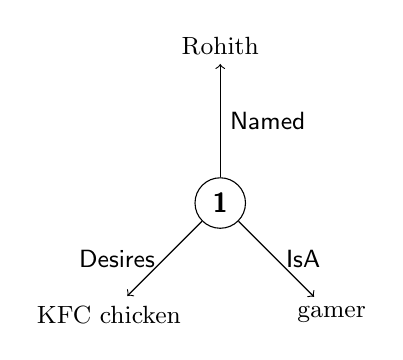
\begin{tikzpicture}[->, node distance=2cm,main node/.style={circle, draw, font=\sffamily\bfseries}]
            \tikzstyle{every node}=[font=\small]
            
              \node[main node] (1) [] {1};
              \node[] (3) [above of=1]{Rohith};
              \node[] (4) [below right of=1] {gamer};
              \node[] (5) [below left of=1] {KFC chicken};
              
            
              \path[every node/.style={font=\sffamily\small}]
                (1) edge node [right] {Named} (3)
                   	edge node [right] {IsA} (4)
                   	edge node [left] {Desires} (5);
                  
            \end{tikzpicture}
\end{subfigure}
\begin{subfigure}[t!]{0.5\textwidth}
	\centering
    \textit{an early man allegedly named Rohith\\a gamer securely established in myth\\he aspired as KFC chicken\\he smarted with gamer thicken\\a noticeable, asleep gamer silversmith}
\end{subfigure}
\caption{Limerick seeded with inspiration}
\label{fig:inspr-lim1}
\end{figure}

\begin{figure}[H]
\centering
\begin{subfigure}[t!]{0.4\textwidth}
	\centering
    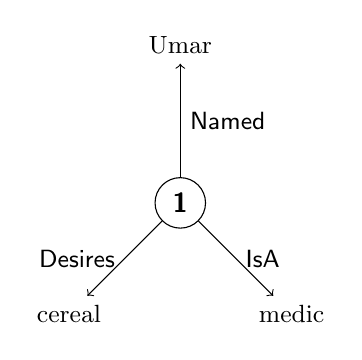
\begin{tikzpicture}[->, node distance=2cm,main node/.style={circle, draw, font=\sffamily\bfseries}]
            \tikzstyle{every node}=[font=\small]
            
              \node[main node] (1) [] {1};
              \node[] (3) [above of=1]{Umar};
              \node[] (4) [below right of=1] {medic};
              \node[] (5) [below left of=1] {cereal};
              
            
              \path[every node/.style={font=\sffamily\small}]
                (1) edge node [right] {Named} (3)
                   	edge node [right] {IsA} (4)
                   	edge node [left] {Desires} (5);
                  
            \end{tikzpicture}
\end{subfigure}
\begin{subfigure}[t!]{0.5\textwidth}
	\centering
    \textit{there be a young medic named Umar\\the attractive man serves behind bar\\say he longs for cereal\\publishes material\\the successful launch washes vintage car}
\end{subfigure}
\caption{Limerick seeded with inspiration}
\label{fig:inspr-lim2}
\end{figure}

\begin{figure}[H]
\centering
\begin{subfigure}[t!]{0.4\textwidth}
	\centering
    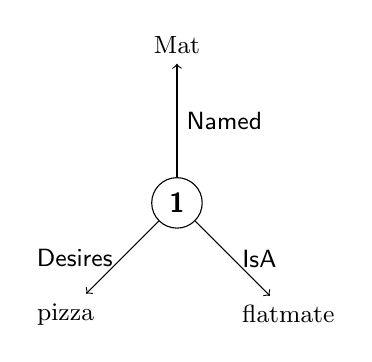
\begin{tikzpicture}[->, node distance=2cm,main node/.style={circle, draw, font=\sffamily\bfseries}]
            \tikzstyle{every node}=[font=\small]
            
              \node[main node] (1) [] {1};
              \node[] (3) [above of=1]{Mat};
              \node[] (4) [below right of=1] {flatmate};
              \node[] (5) [below left of=1] {pizza};
              
            
              \path[every node/.style={font=\sffamily\small}]
                (1) edge node [right] {Named} (3)
                   	edge node [right] {IsA} (4)
                   	edge node [left] {Desires} (5);
                  
            \end{tikzpicture}
\end{subfigure}
\begin{subfigure}[t!]{0.5\textwidth}
	\centering
    \textit{there be a young man named Mat\\long-standing flatmate trims excess fat\\he ambitions vanishes of pizza\\he enters arena\\it all but, humanely, destroys habitat}
\end{subfigure}
\caption{Limerick seeded with inspiration}
\label{fig:inspr-lim3}
\end{figure}

\begin{figure}[H]
\centering
\begin{subfigure}[t!]{0.4\textwidth}
	\centering
    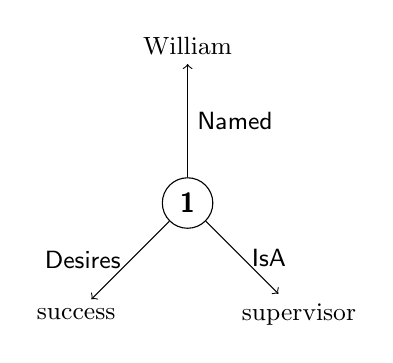
\begin{tikzpicture}[->, node distance=2cm,main node/.style={circle, draw, font=\sffamily\bfseries}]
            \tikzstyle{every node}=[font=\small]
            
              \node[main node] (1) [] {1};
              \node[] (3) [above of=1]{William};
              \node[] (4) [below right of=1] {supervisor};
              \node[] (5) [below left of=1] {success};
              
            
              \path[every node/.style={font=\sffamily\small}]
                (1) edge node [right] {Named} (3)
                   	edge node [right] {IsA} (4)
                   	edge node [left] {Desires} (5);
                  
            \end{tikzpicture}
\end{subfigure}
\begin{subfigure}[t!]{0.5\textwidth}
	\centering
    \textit{there was a primitive man called William\\supervisor thirsted for civilian million\\he interested in success\\a thin man concisely assess\\the father divines man vermilion}
\end{subfigure}
\caption{Limerick seeded with inspiration}
\label{fig:inspr-lim4}
\end{figure}

The point about improving cohesiveness is evident from the second lines of the last penultimate example. Since we knew that the third line would use \textit{'pizza'} in the first of them, the rhyming word chosen for the second line was \textit{'fat'} because it is the most associatively similar. The same goes with \textit{'success'} and \textit{'million'} in the last example and \textit{'cereal'} and \textit{'bar'} in the second example. In the first example, \textit{'myth'} was chosen because it knows that the persona is male and the concept \textit{'man.n'} is two hops away from \textit{'myth.n'} on our knowledge graph (via \textit{'mystery.n'}).

\subsection{Turing-style Tests}
We employ Turing-style tests to assess whether participants can tell human poems apart from ones generated by our system. Five haiku and five limericks were generated \textit{without} inspiration. They were each then shuffled together with five poems sampled from their respective corpora, which were written by humans. 

The poems were put in a survey with answer options as \textit{"Human"}, \textit{"Computer"} and \textit{"Can't tell"}. We also leave space for participants to give their feedback on their decision, which is extremely valuable because it  tells us how we can improve for the future.

Overall the results are promising - every poem generated by our system was thought to have been written by a human by more than 10\% of participants. 

For the haiku, the worst result had 82.16\% of participants realising that it was created by a computer (Figure \ref{fig:haik-test5}). The best result had only 34.34\% realised that it was generated by a computer (Figure \ref{fig:haik-test4}). However, some of the human written poems were also mostly thought to be computer generated. This reduces the integrity of the test because it could mean that the participants were not qualified to take the test due to lack of knowledge about haiku or poor command English. Alternatively, it could be that the human-generated poems were of a relatively poor quality as they were randomly selected.

The limericks results did not look as good. The worst result had 86.99\% of participants realising that it was created by a computer (Figure \ref{fig:lim-test5}). The best result had 73.17\% realised that it was generated by a computer (Figure \ref{fig:lim-test9}). The main reasons for this are that even thought the words were related, the limericks were not cohesive and did not tell a story. We discuss this further in later sections.

The results of the Haiku test are shown in Figures \ref{fig:haik-test1} through \ref{fig:haik-test10} and the limerick test in Figures \ref{fig:lim-test1} through \ref{fig:lim-test10}. The correct answer is shown in \textbf{blue} on the pie charts.

\begin{figure}[H]
\centering
\begin{subfigure}[t!]{0.45\textwidth}
	\centering
    \textit{shape taps on window\\the brightness flares upon\\it causes concern}
\end{subfigure}
\begin{subfigure}[t!]{0.45\textwidth}
	\centering
    \includegraphics[width=70mm]{haik-test1}
\end{subfigure}
\caption{Haiku Turing Test Question 1}
\label{fig:haik-test1}
\end{figure}

\begin{figure}[H]
\centering
\begin{subfigure}[t!]{0.45\textwidth}
	\centering
    \textit{met on September\\she melts frozen me\\like how rain soaks into sea}
\end{subfigure}
\begin{subfigure}[t!]{0.45\textwidth}
	\centering
    \includegraphics[width=70mm]{haik-test2}
\end{subfigure}
\caption{Haiku Turing Test Question 2}
\label{fig:haik-test2}
\end{figure}

\begin{figure}[H]
\centering
\begin{subfigure}[t!]{0.45\textwidth}
	\centering
    \textit{silly confused plants\\harbinger an early spring\\fifty eighth more to come}
\end{subfigure}
\begin{subfigure}[t!]{0.45\textwidth}
	\centering
    \includegraphics[width=70mm]{haik-test3}
\end{subfigure}
\caption{Haiku Turing Test Question 3}
\label{fig:haik-test3}
\end{figure}

\begin{figure}[H]
\centering
\begin{subfigure}[t!]{0.45\textwidth}
	\centering
    \textit{chlorine bleach critique\\element abject force out\\a military source}
\end{subfigure}
\begin{subfigure}[t!]{0.45\textwidth}
	\centering
    \includegraphics[height=55mm]{haik-test4}
\end{subfigure}
\caption{Haiku Turing Test Question 4}
\label{fig:haik-test4}
\end{figure}

\begin{figure}[H]
\centering
\begin{subfigure}[t!]{0.45\textwidth}
	\centering
    \textit{oblong, homeless box\\the dialog like a script\\packs sound in a box}
\end{subfigure}
\begin{subfigure}[t!]{0.45\textwidth}
	\centering
    \includegraphics[height=51mm]{haik-test5}
\end{subfigure}
\caption{Haiku Turing Test Question 5}
\label{fig:haik-test5}
\end{figure}

\begin{figure}[H]
\centering
\begin{subfigure}[t!]{0.45\textwidth}
	\centering
    \textit{summer's solstice\\the voice of the cormorant\\dreams of yesterday}
\end{subfigure}
\begin{subfigure}[t!]{0.45\textwidth}
	\centering
    \includegraphics[height=60mm]{haik-test6}
\end{subfigure}
\caption{Haiku Turing Test Question 6}
\label{fig:haik-test6}
\end{figure}

\begin{figure}[H]
\centering
\begin{subfigure}[t!]{0.45\textwidth}
	\centering
    \textit{an education\\funding university\\a pre-school playgroup}
\end{subfigure}
\begin{subfigure}[t!]{0.45\textwidth}
	\centering
    \includegraphics[width=70mm]{haik-test7}
\end{subfigure}
\caption{Haiku Turing Test Question 7}
\label{fig:haik-test7}
\end{figure}

\begin{figure}[H]
\centering
\begin{subfigure}[t!]{0.45\textwidth}
	\centering
    \textit{unstable condition\\political like a watershed\\state turns to ferment}
\end{subfigure}
\begin{subfigure}[t!]{0.45\textwidth}
	\centering
    \includegraphics[width=70mm]{haik-test8}
\end{subfigure}
\caption{Haiku Turing Test Question 8}
\label{fig:haik-test8}
\end{figure}

\begin{figure}[H]
\centering
\begin{subfigure}[t!]{0.45\textwidth}
	\centering
    \textit{foaming white horses\\rolling in collapse on dunes\\look a jellyfish}
\end{subfigure}
\begin{subfigure}[t!]{0.45\textwidth}
	\centering
    \includegraphics[width=70mm]{haik-test9}
\end{subfigure}
\caption{Haiku Turing Test Question 9}
\label{fig:haik-test9}
\end{figure}

\begin{figure}[H]
\centering
\begin{subfigure}[t!]{0.45\textwidth}
	\centering
    \textit{today was lovely\\i worked and walked carefully\\happened this lately}
\end{subfigure}
\begin{subfigure}[t!]{0.45\textwidth}
	\centering
    \includegraphics[width=70mm]{haik-test10}
\end{subfigure}
\caption{Haiku Turing Test Question 10}
\label{fig:haik-test10}
\end{figure}

\begin{figure}[H]
\centering
\begin{subfigure}[t!]{0.45\textwidth}
	\centering
    \textit{amazingly, antelope stew\\is supposedly better for you\\than a goulash of rat\\or Hungarian cat\\but I guess that you probably gnu}
\end{subfigure}
\begin{subfigure}[t!]{0.45\textwidth}
	\centering
    \includegraphics[height=60mm]{lim-test1}
\end{subfigure}
\caption{Limerick Turing Test Question 1}
\label{fig:lim-test1}
\end{figure}

\begin{figure}[H]
\centering
\begin{subfigure}[t!]{0.45\textwidth}
	\centering
    \textit{there was a strange man named Einstein\\the genius scientist followed the line\\central overtakes the leader\\he polishes off a reader\\a rational person imposes fine}
\end{subfigure}
\begin{subfigure}[t!]{0.45\textwidth}
	\centering
    \includegraphics[height=60mm]{lim-test2}
\end{subfigure}
\caption{Limerick Turing Test Question 2}
\label{fig:lim-test2}
\end{figure}

\begin{figure}[H]
\centering
\begin{subfigure}[t!]{0.45\textwidth}
	\centering
    \textit{at I sighed as I hoped\\for a bike like a Harley I groped\\in my pocket for cash\\and bought something less flash\\then I sat on my moped and moped}
\end{subfigure}
\begin{subfigure}[t!]{0.45\textwidth}
	\centering
    \includegraphics[height=55mm]{lim-test3}
\end{subfigure}
\caption{Limerick Turing Test Question 3}
\label{fig:lim-test3}
\end{figure}

\begin{figure}[H]
\centering
\begin{subfigure}[t!]{0.45\textwidth}
	\centering
    \textit{to compose a sonata today\\don't proceed in the old fashioned way\\with your toes on the keys\\bang the floor with your knees\\oh how modern critics will say}
\end{subfigure}
\begin{subfigure}[t!]{0.45\textwidth}
	\centering
    \includegraphics[height=60mm]{lim-test4}
\end{subfigure}
\caption{Limerick Turing Test Question 4}
\label{fig:lim-test4}
\end{figure}

\begin{figure}[H]
\centering
\begin{subfigure}[t!]{0.45\textwidth}
	\centering
    \textit{the weather uproots devilwood\\evergreen roots autumn bulb wood\\it maintains stance\\has one clear-cut chance\\possibility strengthens position good}
\end{subfigure}
\begin{subfigure}[t!]{0.45\textwidth}
	\centering
    \includegraphics[height=58mm]{lim-test5}
\end{subfigure}
\caption{Limerick Turing Test Question 5}
\label{fig:lim-test5}
\end{figure}

\begin{figure}[H]
\centering
\begin{subfigure}[t!]{0.45\textwidth}
	\centering
    \textit{there was a young person called Smarty\\who sent out his cards for a party\\so exclusive and few\\were the friends that he knew\\that no one was present but Smarty}
\end{subfigure}
\begin{subfigure}[t!]{0.45\textwidth}
	\centering
    \includegraphics[height=60mm]{lim-test6}
\end{subfigure}
\caption{Limerick Turing Test Question 6}
\label{fig:lim-test6}
\end{figure}

\begin{figure}[H]
\centering
\begin{subfigure}[t!]{0.45\textwidth}
	\centering
    \textit{the middle-aged man from France\\while communication keeps his stance\\his position is in love\\emotion is ugly like a cancer above\\he logically does not advance}
\end{subfigure}
\begin{subfigure}[t!]{0.45\textwidth}
	\centering
    \includegraphics[height=50mm]{lim-test7}
\end{subfigure}
\caption{Limerick Turing Test Question 7}
\label{fig:lim-test7}
\end{figure}

\begin{figure}[H]
\centering
\begin{subfigure}[t!]{0.45\textwidth}
	\centering
    \textit{the bold chlorine contaminates water\\the landscape gives short birth to daughter\\binary compounds crosses lagoon\\chemical element goes up in balloon\\derives inspiration underwater}
\end{subfigure}
\begin{subfigure}[t!]{0.45\textwidth}
	\centering
    \includegraphics[width=60mm]{lim-test8}
\end{subfigure}
\caption{Limerick Turing Test Question 8}
\label{fig:lim-test8}
\end{figure}

\begin{figure}[H]
\centering
\begin{subfigure}[t!]{0.45\textwidth}
	\centering
    \textit{there is a young, fine man called Ricky\\he is as dark-haired as a trainer sticky\\he wants to slumber\\he gets a wrong number\\deep sleeps quite tricky}
\end{subfigure}
\begin{subfigure}[t!]{0.45\textwidth}
	\centering
    \includegraphics[width=60mm]{lim-test9}
\end{subfigure}
\caption{Limerick Turing Test Question 9}
\label{fig:lim-test9}
\end{figure}

\begin{figure}[H]
\centering
\begin{subfigure}[t!]{0.45\textwidth}
	\centering
    \textit{a talkative tourist named Margot\\was handed a plate of escargot\\at a fancy French feast\\then her chattering ceased\\and the whole crowd soon heard her new car go}
\end{subfigure}
\begin{subfigure}[t!]{0.45\textwidth}
	\centering
    \includegraphics[width=60mm]{lim-test10}
\end{subfigure}
\caption{Limerick Turing Test Question 10}
\label{fig:lim-test10}
\end{figure}

\subsection{Quality of English}
We mentioned at the start of this paper that poetry is meant to convey a particular message. We argued that we need control over syntax and semantics of language to achieve this goal, and that it comes before attempting to use poetic features.

\subsubsection{Vocabulary and Word Selection}
The vocabulary of the system is dispersed among the third-party and internal sources used.
\begin{description}
\item[WordNet] ~117,000 words
\item[CMUPD] ~133,000 words
\item[FrameNet] ~13,000 words
\item[Knowledge Network] 28,802 words
\item[SimpleNLG Lexicon]: 6317 words
\end{description}

The most important of these are the last three in the list because they come with semantic information on the usage, inflections and associations of words. The average vocabulary of native English speakers is 20,000-35,000\cite{vocab}, so there is still plenty of room for improvement. 

It is worth noting that there is little to no scientific or colloquial vocabulary. Names of people and places in our knowledge network is also limited.

Given the limited repetition of words in the poems, this vocabulary size is sufficient. The Turing Test results did not indicate any issues with vocabulary being too basic for a human author.

\subsubsection{Grammar and Sentence Structure}
The grammatical capabilities are mainly governed by FrameNet and SimpleNLG. FrameNet gives the instruction on how to build a sentence from a single word, while SimpleNLG can be used to follow those instructions. This approach enables us to build upwards from words to phrases to complex sentences based on first principles of structuring a sentence with subjects, actions, objects and indirect objects.

This gives us the ability to generate many types of sentences for any purpose. The initial structure of every line of poetry created by this system has correct grammar and is only broken for poetic license. As a result, the grammar produced by this system is of a higher quality compared to many previous works (see Section \ref{sec:related_work}) and yet is flexible enough to be unpredictable.

Comments on the Turing Tests did not condemn the grammar of the computer generated poetry. Some comments did admonish the grammar of human generated poetry, indicating that it was a factor that participants looked out for. One comment even said \textit{"The grammar seems too off to be poetic license."} about a human generated poem. This justifies our content-first approach.

The amount of vocabulary used effectively is somewhat limited by the fact that we translate a relation (of which there are relatively few types) to phrases. We use the general takes and receives action relations to spread our usable vocabulary as wide as possible, but quality will significantly improve if we get more relations like in ConceptNet\cite{liu2004conceptnet}.

One major point of feedback from the Turing Tests was the inability for this system to carry out \textit{enjambment} - letting sentences overflow into multiple lines. Given our process of building from first principles, we build noun phrases and verb phrases that get \textit{realised} into a full sentence. We can simply split these phrases over multiple lines to achieve enjambment. This is particularly important for poems with very short syllable counts, such as haikus. 


\subsection{Creativity and Cohesiveness}
Poems are \textit{creative} works, which means that they should at least be \textit{non-deterministic}.

We generated 100 poems where 50 were given the same \textit{word} as inspiration and 50 the same \textit{relation} as inspiration.

Each poem was very different in the case of the single word inspiration. When given the same relation as inspiration, the first line was always a direct translation as per Section \ref{sec:build}, which means that there was \textit{some} overlap in that line, but little in the others.

Furthermore, if the tail of the given relation is a word with very few rhyming candidates then following lines may end up being similar because of lack of choices for words. However, there is enough non-determinism, thanks to a large knowledge network and the randomness introduced in the rephrasing processes, for there to be consistent variation.

\subsubsection{Knowledge as Creativity}
One philosophy of creativity is that it is an amalgamation of knowledge and experience. Our system has its semantic network of common-sense (Section \ref{sec:common-sense}) that fills this role. It has precisely 203,324 relations between 28,802 unique concepts (compared to de Smedt's Perception with ~9,000 relations across ~4,000 concepts) from high-quality and dependable sources. There are more resources, such as ConceptNet, that could be used to extend this knowledge base in the future.

A third of all relations are of the most general \textit{RelatedTo} type, which is only really useful for cohesiveness throughout the poem and do not help building relations between persona. More specific understanding of the relations between words will increase the variation, and therefore creativity, of the system.


\subsubsection{Cohesiveness}
The problem of a cohesive theme is a very important one. Many decisions made by participants on the Turing test were based on the extent to which words in the poem were related to each other. The haiku in Figure \ref{fig:haik-test7} mentions words on the theme of education but are not related temporally or any other way. This haiku still fooled many, and the reason given was that they did not expect such cohesiveness from a computer. Human poems were also admonished for their lack of cohesiveness and therefore thought to be computer-generated.

Cohesiveness in this system is achieved on a word-by-word basis by finding associatively similar concepts in the knowledge graph. At the moment, the context concept nodes include those in the lines immediately surrounding the one being built. This gives a ladder effect to the cohesiveness; we can go from one topic to another but may end up far away from the original by the end of the poem. This is a big reason the limericks performed poorly compared to the haiku, according to feedback on the Turing test.

A better strategy could be to attain a circular effect, whereby we aim to return to the original concept that we started with by the end of the poem. Or we have a star effect, where one concept anchors the entire poem. Thorough experimentation with different strategies will be required to uncover a consistently effective approach.

Many human poems were lauded for their story-telling; a temporally consecutive series of events. Further investigation into strategies that utilise tense and aspect together with cohesiveness may be the final piece in the puzzle for automatic generation of poetry, especially if it is able to cope with long poems that include many stanzas.


\subsection{Performance}
The timings taken to generate 10 haikus and 10 limericks without inspiration are seen in Table \ref{tab:gen}. On average, a limerick takes \textbf{322.75} seconds and a haiku takes \textbf{12.53} seconds to create.

\begin{table}
\centering
    \begin{tabular}{|l|l|}
    \hline
    Limerick & Haiku  \\ \hline
    291.992  & 21.365 \\
    241.588  & 12.608 \\
    50.754   & 14.134 \\
    863.205  & 13.066 \\
    16.115   & 10.385 \\
    369.568  & 9.384  \\
    491.374  & 10.889 \\
    584.955  & 9.145  \\
    290.491  & 15.148 \\
    27.447   & 9.137  \\ \hline
    \end{tabular}
\caption{Timings for generating 10 haikus and 10 limericks}
\label{tab:gen}
\end{table}

\subsubsection{Delay when Finding Rhymes}

It is intuitive that longer poems take more time to compose. The less obvious trend is that adherence to a rhyme scheme greatly increases processing time because choosing the most associatively similar (see Section \ref{sec:assoc-sim}) pair of words when rephrasing for rhyme, as described in Section \ref{sec:guarantee-rhyme}, causes the greatest delay.

Suppose we want to choose the best word in context to rhyme with \textit{'cheese'}. The call to the RhymeBrain API\cite{rhymebrain} takes $0.599$ seconds and returns $117$ candidate rhymes. If we assume we have $10$ contextual words to compare with then we require $1170$ graph lookups. In most cases lookup converges to a maximum depth of $1$ eventually, which has an average lookup time of $0.0043$. However, there may be some lookups of maximum depth of $2$ or $3$ before converging, which have average times of $0.228$ and $1.691$ seconds respectively. 

Therefore, the time to complete our \textit{'cheese'} example is at best\\ $1170*0.0043 + 0.599  = 5.63$\\ seconds but could potentially take up to roughly\\ $50*1.691 + 120*0.228 + 1000*0.0043 + 0.599  = 116.809$\\ seconds just to choose one word with machine specifications in Appendix \ref{sec:specs}.

There are several ways this can be improved with threading, caching, optimising the shortest path algorithm and reducing API calls. However, this implementation is inherently long-winded because we are getting the rhyme words \textit{first}, and then finding the most contextually appropriate. 

A more efficient implementation would be to store the rhyme phoneme patterns, as in Section \ref{sec:rhyme}, in each node of the knowledge network. We then start from each context node and do a breadth first search for the nearest node with the required rhyme phoneme pattern. For further optimisation, we could create a thread for each context node and perform this process concurrently.

This removes the need for an API call and for the shortest path associative similarity altogether, significantly reducing time and memory complexity.

\subsubsection{SimpleNLG via JPype}

Another sub-optimal implementation is that the Natural Language Generation library that we use in this project is SimpleNLG, a \textit{Java} library. This is made possible by launching a JVM via JPype, which also allows us to run the library and access its objects. Naturally, it will be more efficient to use local Python implementation.

% ------------------------------------------------------------------------


%%% Local Variables: 
%%% mode: latex
%%% TeX-master: "../thesis"
%%% End: 
